\def\lecturenumber{07}
\documentclass[11pt,a4paper]{article}
\usepackage[T1]{fontenc}
\usepackage[utf8]{inputenc}
\usepackage{lmodern}
\usepackage[margin=19mm,top=21mm,bottom=21mm,headheight=15pt]{geometry}
\usepackage{amsmath,amssymb,booktabs,array,graphicx,microtype}
\usepackage[dvipsnames]{xcolor}
\usepackage{enumitem,fancyhdr,listings,tcolorbox}
\usepackage[colorlinks=true,linkcolor=MidnightBlue,urlcolor=MidnightBlue]{hyperref}
\definecolor{courseblue}{HTML}{164B69}
\definecolor{pale}{HTML}{F0F5F7}
\pagestyle{fancy}
\fancyhf{}
\fancyhead[L]{\small\sffamily\color{courseblue}VALIDATED COMPUTING}
\fancyhead[R]{\small\sffamily Lecture \lecturenumber}
\fancyfoot[L]{\footnotesize Expanded lecture notes \textbullet\ October 2026}
\fancyfoot[R]{\footnotesize\thepage\ / 6}
\renewcommand{\headrulewidth}{0.4pt}
\setlength{\parindent}{0pt}
\setlength{\parskip}{5.5pt plus 1pt}
\setlength{\emergencystretch}{1.5em}
\setlist[itemize]{leftmargin=1.5em,itemsep=3pt,topsep=3pt}
\setlist[enumerate]{leftmargin=1.7em,itemsep=5pt,topsep=4pt}
\lstset{language=Python,basicstyle=\small\ttfamily,keywordstyle=\color{courseblue}\bfseries,
 commentstyle=\color{OliveGreen},stringstyle=\color{BrickRed},showstringspaces=false,
 columns=fullflexible,keepspaces=true,frame=single,rulecolor=\color{black!18},
 backgroundcolor=\color{black!2},aboveskip=6pt,belowskip=6pt,breaklines=true,
 xleftmargin=5pt,xrightmargin=5pt,framesep=5pt}
\newcommand{\R}{\mathbb R}
\newcommand{\fl}{\operatorname{fl}}
\newcommand{\abs}[1]{\left|#1\right|}
\newcommand{\heading}[2]{\section*{\color{courseblue}#1}\vspace{-4pt}{\small\sffamily\color{black!65}#2}\par\vspace{3pt}}
\newcommand{\opening}[2]{{\Large\sffamily\bfseries\color{courseblue}Lecture \lecturenumber\quad #1\par}\vspace{5pt}{\small #2}\par}
\newtcolorbox{question}[1]{colback=pale,colframe=courseblue!55,boxrule=0.4pt,
 arc=1mm,left=7pt,right=7pt,top=4pt,bottom=4pt,title={#1},fonttitle=\bfseries\small,
 coltitle=courseblue,colbacktitle=pale}
\newcommand{\reading}[1]{{\footnotesize\textbf{Reading and notebook.} #1\par}}
\hypersetup{pdfauthor={Validated Computing course},pdfsubject={Expanded introductory lecture notes with questions and exercises}}

\hypersetup{pdftitle={Lecture 07: Derivatives and better enclosures}}
\begin{document}
\opening{Derivatives and better enclosures}{Prerequisites: Lectures 04--06 and the mean value theorem.\newline
Goal: improve range bounds with derivatives and report exactly what an adaptive calculation has achieved.}
\heading{1. Enclose all slopes, then use the mean value theorem}{0--15 minutes: derive a new inclusion formula}
Subdivision improves many natural interval extensions, but it ignores useful
information about how the function changes. A derivative bound can relate a
value at one point to values across a whole interval. The derivative must be
bounded everywhere in that interval; an accurate derivative at one point is
not enough.

Let $f$ be continuously differentiable on a neighborhood of $X=[a,b]$.
Choose an exact centre $m\in X$. Suppose $C$ encloses $f(m)$ and $D$ encloses
$f'(x)$ for every $x\in X$. Then the \emph{mean-value enclosure} is
\[
               f(X)\subseteq M(X):=C+D(X-[m,m]).
\]
\textbf{Proof.} Fix $x\in X$, with $x\ne m$. The mean value theorem gives
$f(x)=f(m)+f'(\xi)(x-m)$ for some $\xi$ between $m$ and $x$. Since $\xi\in X$,
the derivative belongs to $D$; the other two quantities belong to their stated
enclosures. Interval composition proves inclusion. For $x=m$, the displacement
is zero and the result follows from $f(m)\in C$.

The point $\xi$ depends on $x$ and is usually unknown. The proof works because
$D$ covers every possible choice. The midpoint $m=(a+b)/2$ minimizes the
largest distance to an endpoint, making it a useful default centre. Any
specified point in $X$ is permitted by the theorem.

\textbf{Worked example.} Continue with $f(x)=x(1-x)$, now on $X=[1/4,3/4]$.
Its derivative is $1-2x$, so $D=[-1/2,1/2]$. At $m=1/2$ the exact function
value is $1/4$. Thus
\[
 M(X)=[1/4,1/4]+[-1/2,1/2]\,[-1/4,1/4]=[1/8,3/8].
\]
The natural product gives $[1/16,9/16]$, while the true range is
$[3/16,1/4]$. The new bound is narrower, although still not exact. The
independent choices of slope and displacement explain the remaining excess.

\begin{question}{Which premises belong to which computation?}
Identify $X$, $m$, $C$, and $D$ in the example. Which use exact rational
arithmetic? If evaluating $f(m)$ required a transcendental function, could
we replace $C$ by its nearest-rounded midpoint? Explain the needed guarantee.
\end{question}

\textbf{A derivative is part of the specification.} A callback named
\texttt{derivative} is not automatically correct. Its expression must be the
derivative of the same real function, and its interval evaluation must enclose
that derivative on the whole input. Lecture 08 will automate differentiation
rules while preserving this distinction between a formula and its enclosure.

\newpage
\heading{2. Compute both bounds and retain their intersection}{15--31 minutes: exact code and a counterexample to automatic improvement}
Two independently valid enclosures of the same range can be intersected.
The result is contained in both. An empty intersection on a nonempty domain
signals inconsistent premises or a programming error; it is not evidence that
a defined function has an empty range.

Here is a small evaluator specifically for $x(1-x)$ on subintervals of $[0,1]$.
Endpoints are \texttt{Fraction} objects. The four-product rule from Lecture 04
handles the signs of both slopes and displacements.
\begin{lstlisting}
from fractions import Fraction

def interval_product(X, Y):
    a, b = X
    c, d = Y
    products = [a*c, a*d, b*c, b*d]
    return min(products), max(products)

def combined_bound(a, b):
    assert 0 <= a <= b <= 1
    natural = (a * (1-b), b * (1-a))
    center = (a + b) / 2
    value = center * (1-center)
    slopes = (1-2*b, 1-2*a)
    displacement = (a-center, b-center)
    lower, upper = interval_product(slopes, displacement)
    centered = (value + lower, value + upper)
    result = (max(natural[0], centered[0]),
              min(natural[1], centered[1]))
    if result[0] > result[1]:
        raise ValueError("Inconsistent enclosures")
    return result

assert combined_bound(Fraction(1, 4), Fraction(3, 4)) == (
    Fraction(1, 8), Fraction(3, 8))
\end{lstlisting}

\textbf{The centred form can be worse.} For $g(x)=x^2$ on $[0,1]$, a sharp
square gives the exact range $[0,1]$. The midpoint calculation instead gives
\[
 [1/4,1/4]+[0,2],[-1/2,1/2]=[-3/4,5/4].
\]
It remains valid; intersection recovers $[0,1]$. Using only $g'(1/2)=1$ would
give $[-1/4,3/4]$, which misses $g(1)=1$ and is invalid. A narrower answer
is valuable only after its inclusion argument has been established.

\begin{question}{A centre moves when the interval changes}
Why does the mean-value proof establish validity separately on each interval,
without proving that re-centred bounds are nested under subdivision? Which
property does intersection guarantee on each individual input?
\end{question}

\newpage
\heading{3. Derivative signs can settle a range exactly}{31--46 minutes: monotonicity and endpoint values}
If a valid derivative enclosure satisfies $D\subseteq[0,\infty)$, then $f$
is nondecreasing on $X$. For $x<y$, the mean value theorem gives
$f(y)-f(x)=f'(\xi)(y-x)\geq0$. Similarly, a nonpositive derivative proves
that $f$ is nonincreasing. A derivative bounded strictly away from zero
proves strict monotonicity, a property we will use for uniqueness of roots.

For a nondecreasing function, the exact range is $[f(a),f(b)]$. If $A$ and
$B$ enclose these endpoint values, $[\inf A,\sup B]$ is a valid range bound.
For a nonincreasing function, use $[\inf B,\sup A]$. Taking the hull of
both endpoint enclosures is also safe in either case, though sometimes wider.
Endpoint evaluation itself still needs exact or outward-rounded arithmetic.

For $f(x)=x(1-x)$ on $[0,1/4]$, the derivative lies in $[1/2,1]$.
Consequently the range is $[f(0),f(1/4)]=[0,3/16]$. The natural product
$[0,1/4]$ loses information that the derivative sign recovers immediately.
On $[0,1]$, however, $D=[-1,1]$ makes this test inconclusive.

Split the latter domain at $1/2$. The left derivative enclosure is $[0,1]$,
and the right is $[-1,0]$. The first half is nondecreasing and the second
nonincreasing. Each half has range $[0,1/4]$, so their hull recovers the
exact global range. Zero at an endpoint of $D$ does not prevent a
\emph{nonstrict} monotonicity argument.

\begin{center}
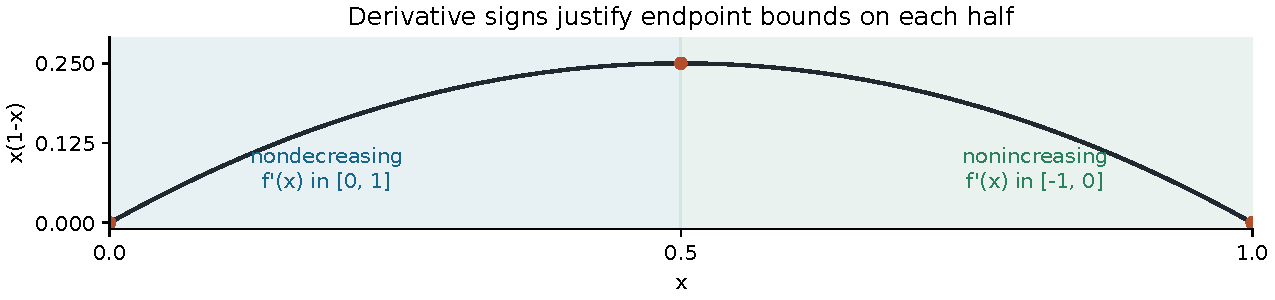
\includegraphics[width=0.92\linewidth]{figures/monotone_pieces.pdf}
\end{center}

\textbf{An inconclusive sign test is not a turning-point test.} A wide
enclosure may contain both signs even if the actual derivative is always
positive. Conversely, if the derivative vanishes somewhere, the function may
still be strictly increasing: $x^3$ is an example. Our sufficient test does
not classify every possible function.

\begin{question}{Explain what endpoint sampling is missing}
Both endpoints of $x(1-x)$ on $[0,1]$ equal zero. Why is their hull an
invalid range bound there? What additional theorem makes the endpoint method
valid on each half? Distinguish evaluating endpoints from proving monotonicity.
\end{question}

For functions with several turning regions, one can apply the sign test
piece by piece, using another valid evaluator where it fails. Every retained
piece still needs a range enclosure. A mixed strategy is legitimate because
coverage and local inclusion, rather than uniformity of method, justify the hull.

\newpage
\heading{4. An adaptive loop with a visible invariant}{46--63 minutes: read the algorithm and trace one split}
Maintain pieces covering the original domain, each carrying a valid image.
Split the piece with the widest image first. The target is that \emph{every
local image} has width at most $\tau$. This function uses exact rational
endpoints, a positive rational tolerance, and a positive integer budget.
\begin{lstlisting}
def make_piece(a, b):
    lower, upper = combined_bound(a, b)
    return a, b, lower, upper

def adaptive_cover(tolerance, max_pieces):
    if tolerance <= 0 or max_pieces < 1:
        raise ValueError("Need positive tolerance and budget")
    pieces = [make_piece(Fraction(0), Fraction(1))]
    while True:
        widest_index = 0
        for index in range(1, len(pieces)):
            width = pieces[index][3] - pieces[index][2]
            widest = pieces[widest_index]
            if width > widest[3] - widest[2]:
                widest_index = index
        a, b, lower, upper = pieces[widest_index]
        if upper - lower <= tolerance:
            return pieces, "resolved"
        if len(pieces) >= max_pieces:
            return pieces, "budget_exhausted"
        if a == b:
            return pieces, "cannot_split"
        center = (a + b) / 2
        left = make_piece(a, center)
        right = make_piece(center, b)
        pieces.pop(widest_index)
        pieces.append(left)
        pieces.append(right)
\end{lstlisting}

The loop's invariant has two parts: the domains cover $[0,1]$, and every
stored image encloses the function on its associated domain. Replacing one
closed interval by its two closed halves preserves coverage. Evaluating both
children before removing the parent avoids returning a partially updated cover
if an evaluation fails. The invariant proves the validity of the current hull
at every successful return, including a budget-limited return.

\begin{question}{Trace the first two iterations}
For $\tau=1/16$, compute the parent image and the two child images by hand.
If the budget is two pieces, which status is returned? Does that status say
the current range bound is invalid, or that the local target was not met?
\end{question}

This small example fixes both the function and original domain to keep the
loop readable. The notebook generalizes them to evaluator and domain arguments.
The choice of the widest image affects efficiency; the coverage proof does not
depend on choosing the optimal piece.

\newpage
\heading{5. Interpret the stopping condition quantitatively}{63--77 minutes: distinguish variation from excess width}
Form the global hull only after retaining all pieces, including difficult
ones. The following code continues the previous excerpts in the same session.
It also checks coverage using the exact endpoints, not the drawing.
\begin{lstlisting}
pieces, status = adaptive_cover(Fraction(1, 16), 128)
pieces.sort()
assert pieces[0][0] == 0 and pieces[-1][1] == 1
for index in range(len(pieces) - 1):
    assert pieces[index][1] == pieces[index+1][0]
lower, upper = pieces[0][2], pieces[0][3]
for a, b, local_lower, local_upper in pieces:
    lower = min(lower, local_lower)
    upper = max(upper, local_upper)
    assert local_upper - local_lower <= Fraction(1, 16)
assert status == "resolved"
assert lower <= 0 and upper >= Fraction(1, 4)
print(status, len(pieces), str(lower), str(upper))
\end{lstlisting}

\textbf{What accuracy follows?} Suppose $f$ is continuous on a compact
domain, and every nonempty covering piece has a valid image $[l_i,u_i]$
of width at most $\tau$. Write $L=\min_i l_i$, $U=\max_i u_i$, and let
$f_{\min},f_{\max}$ be the true extrema. Then
\[
       0\le f_{\min}-L\le\tau,\qquad
       0\le U-f_{\max}\le\tau.
\]
For the first inequality, choose a piece attaining $L$ and any point $x$ in
it. Its image gives $f(x)\le L+\tau$. Thus
$L\le f_{\min}\le f(x)\le L+\tau$. The upper-bound proof is analogous.
This is a useful error guarantee obtained without knowing the true extrema.

The criterion is sufficient, not necessary. An evaluator may already return
the exact global range while some local image widths exceed $\tau$. For
$f(x)=x$ on $[0,1]$, the global width is always at least one; subdivision
can still make every local image arbitrarily narrow. Do not replace the
local target by a global-width target without changing the mathematical question.

\textbf{What if refinement stalls?} A budget limit leaves a valid hull but
does not establish the inequalities above unless all local widths actually
meet the target. A point domain with a wide machine image cannot be split;
arithmetic precision or the evaluator needs attention. More generally, an
arbitrary valid evaluator need not become sharp on smaller inputs, so universal
termination is not promised.

\begin{question}{Write a precise result sentence}
Report what ``resolved with $\tau=1/16$'' proves about the two global endpoints.
Then write a different sentence for ``budget exhausted.'' Explain why neither
status by itself asserts the existence or number of roots.
\end{question}

\newpage
\heading{6. Exercises and a range-certificate audit}{77--90 minutes: choose two in class; complete the rest independently}
\begin{enumerate}
\item \textbf{A sharper bound, with all premises.} For $f(x)=x(1-x)$ on
$[1/4,3/4]$, derive the natural and mean-value bounds and their intersection.
Find the exact range using the vertex form. Explain why a nonempty
intersection checks consistency but does not prove that a supplied derivative
formula is correct.

\item \textbf{A derivative shortcut that fails.} For $g(x)=x^2$ on $[0,1]$,
derive the centred enclosure using $D=[0,2]$, then using the invalid choice
$D=[1,1]$. Identify a missed function value in the second result. Why could
sampling only at the midpoint fail to reveal the mistake?

\item \textbf{Monotonicity without a strictly positive slope bound.}
For $g(x)=x^3$ on $[-1,1]$, use $g'(x)=3x^2$ and a sharp square to obtain
$D=[0,3]$. What range follows from monotonicity? Does this derivative test
alone prove strict increase? Give a separate algebraic reason that $x^3$ is
strictly increasing despite its zero derivative at zero.

\item \textbf{Audit the budget.} Run the adaptive code with
$\tau=1/10^6$ and a budget of two pieces. Check coverage and the global hull.
Explain why increasing the budget is different from increasing arithmetic
precision in this exact-rational example. State a correct conclusion even
if the requested local widths remain unattained.

\item \textbf{A stopping theorem, not a picture.} Prove the upper-endpoint
error inequality on page 5 by choosing a piece attaining $U$ and any point
in that piece. Why must every local image be narrow? If one difficult piece
is discarded, which step of the global argument becomes unavailable?
\end{enumerate}

\textbf{Selected checks.} Exercise 1: the bounds are $[1/16,9/16]$ and
$[1/8,3/8]$, with intersection $[1/8,3/8]$; the true range is
$[3/16,1/4]$. Exercise 2: $[-3/4,5/4]$ is valid, while
$[-1/4,3/4]$ misses $g(1)$. Exercise 3: the range is $[-1,1]$.
For $y>x$, $y^3-x^3=(y-x)(y^2+xy+x^2)>0$, since the quadratic factor
can vanish only when $x=y=0$. Exercise 4: the two domains are $[0,1/2]$
and $[1/2,1]$; both images are $[0,7/16]$, so the hull is $[0,7/16]$.
The status is \texttt{budget\_exhausted}. Exercise 5: on a piece attaining
$U$, any value satisfies $U-\tau\le f(x)\le f_{\max}\le U$.

\begin{question}{Exit ticket: identify the proof carried by the data}
List the original domain, the cover, the function and derivative evaluators,
the local image bounds, the global hull, and the actual stopping status.
Which entries justify inclusion, and which justify the requested accuracy?
Explain why a plot can help inspect this information but cannot replace it.
\end{question}

The next lecture constructs derivatives from elementary rules instead of
requiring a hand-derived formula for each example. It will still distinguish
an approximate derivative value from an enclosure valid on a whole interval.
Run the excerpts here in order; only Python's standard library is required.

\reading{Companion: \texttt{notebooks/07\_better\_enclosures.ipynb} and Lab 07.
Tucker, \emph{Validated Numerics} (2011), \S\S3.2--3.3, pp.~55--59;
\S3.1 supplies the graph-enclosure viewpoint.}
\end{document}
